\section{Our Approach}
In this section, we introduce a probabilistic graphical model of repositories
and the inference of it. In addition, we explore the method of how to map 
the code file distributions to the hierarchical taxonomy.
\subsection{Model for Repository}
\label{sec:method}
%\JK {why we design the model like this? explain it with examples.}
Firstly, we will introduce the intuation of this model with the problems
we listed in \secref{sec:pro} about \exref{ex-bear1}. As is known that
programming languages are artificial languages which are different from
natural languages. They have specific grammar and structures. Let's have a
look at how programmers write these code files. 
\begin{itemize}
\item For code part, programmers intend select the words with use meaningful
semanic, but tese words have to effected by the speical grammer of the specific
programming language.
\item For comment part, this is a natural language part where programmers
talk to himself and other readers, i.e. {\it /* Get and return 
the current wall-time in ticks since boot. */} in ``clock.c''. Of course,
these text are in special area of programming.
\item For commits, programmers usually have to consider what has been done
during this change, this is directly related to the files it touches. In addition,
according to the special usage of commit, some words like ``fix'', ``bug'' will 
also apper inside.
\end{itemize}

We don't have labeled code data, but there are plenty of labeled natural language text
of programming area on website, like {\it Stack overflow}. If we can extract
the corresponding natural language semantic part of code files, we can take
advantage of those labeled text to classify what semantics the code files are.


To mine the topics of repositories, we have to get a comprehension of the 
relationships between the topics of different part of the repositories.
Figure \ref{fig:spet} shows the probabilistic graphical representation of the 
source code system. In this figure, the left part represents one check in 
message and the right part represents a source code file. The variable $a$ 
between these two files means whether they are related to each other.
\begin{figure}[h]
\begin{center}
\includegraphics[width=0.7\columnwidth]{figure/seprate.eps}
\caption{Graphical Model for Code Repository.
d:file, z:topic, w:word, l:language, c:commit, a:connection}
\label{fig:spet}
\end{center}
\end{figure}

We simulate the generation process of the source code repositories with some 
simple assumptions:
For each document $d_m$, the topic of it follows multinorminial distribution $z_{i,m} \sim Multi(z|d_m)$.
Each words, both identifier from code and normal words from comments, also 
follow multinorminial distribution when given the topic. 
One one hand, comments are more likely to be netural languages that the coder used to explain the topics
of those files, the generation os comments are just decided by the topics $w_{j,m} \sim Multi(w|z_{j,m})$. 
On the other hand, the identifier of code are from the languages
of computer, they could also be influenced by the programming 
language itself, which is depicted like $w_{i,m} \sim Multi(w|z_{i,m},l)$.

The generation of commit messages are different from code. 
There is a ``many to many'' relationship between code files and commit messages.
One code file may have a series of commit messages and one commit message may touch
several code files. We make the assumption that they follow one Bernoulli distirbution
$a_{u,m}\sim Bernoulli(a|c_u,d_m)$. Since the topics of one commit message 
can be decided by what is done by this commit. Actually we simplify the reasons 
into two main part, the topics of those files it changed and the commit itself.
\begin{itemize}
\item For the words that is decided by the code files it touches, they are 
generated with two multinorminial distributions $z_{n,u}\sim Multi(z|D,a)$ and 
$w_{n,u} \sim Multi(w|z_{n,u})$ 
\item For those decided by the commit itself, we assume that that words 
follow multinorminial distribution $w_{n,u} \sim Multi(w|c_u)$ 
\end{itemize}

Given the representation of the model, one repository can be generated with the 
following process.

\begin{itemize}
\item \textcolor{red}{For each document $d_m$ which is under a set of directories $Dir$}
\begin{itemize}
\item \textcolor{red}{Draw a connection $b_{m}\sim Bernoulli(b|d_m,Dir)$}
\end{itemize}
\item \textcolor{red}{For each identifier token $w_i$ in a document $d_m$ which is under a set of directories $Dir$,}
\begin{itemize}
\item \textcolor{red}{Draw a topic $z_{i,m} \sim Multi(z|d_m,b_m,Dir)$}
\item Draw an identifier $w_{i,m} \sim Multi(w|z_{i,m},l)$
\end{itemize}
\item For each comment token $w_j$ in a document $d_m$,
\begin{itemize}
\item Draw a topic $z_{j,m} \sim Multi(z|d_m)$
\item Draw an token $w_{j,m} \sim Multi(w|z_{j,m})$
\end{itemize}
\item For each check in message $c_u$ and document $d_m$ 
\begin{itemize}
\item Draw a connection $a_{u,m}\sim Bernoulli(a|c_u,d_m)$
\end{itemize}
\item For each token $w$ of check in message $c$, as well as all the source code 
files set $D$ and the connection matrix $a$
\begin{itemize}
\item Draw a topic $z_{n,u}\sim Multi(z|D,a)$
\item Draw a token $w_{n,u} \sim Multi(w|z_{n,u},c_u)$ 
\end{itemize}
\end{itemize}

The target result we want is a combination of the topic distribution of the 
source code documents:

\textcolor{red}{$p(topic|document, directory)=p(z|d, Dir)$.}

We can easily find that it comes from two different parts, code files
and commit messages.

Since the words distributions of codes $p(w|z_{i,m},l)$ and commits $p(w|z_{n,u},c_u)$ 
are both decided by two different part, we made the assumption as \equref{equ:split}. 
\begin{align}
\label{equ:split}
\begin{split}
p(w|z_{i,m},l)&=\eta p(w|z_{i,m})+(1-\eta) p(w|l)\\
p(w|z_{n,u},c_u)&=\lambda p(w|z_{n,u})+(1-\lambda) p(w|c_u)\\
\end{split}					
\end{align}

For the topic distribution of one commit message $p(z|D,a)$, since it is decided by 
code files it touches, we model those code files as fair contributers. In other words,
if one commit message only touches one code file, the topic of it is totally decided
by the very code file; if one commit message touches ten code files, each file contributes
$1/10$ of its topic distribution to the commit message.
\begin{align} 
\begin{split}
p(z|D,a)=\sum _{d_m \in D }{ p(z|d_m,a_{u,m})}=\sum _{d_m \in D }\xi_{u,m} {p(z|d_m)}\\
\end{split}					
\end{align}
where 
\[\xi_{u,m}=\frac{a_{u,m}}{\sum _{m}{a_{u,m}}}\]

\textcolor{red}{
\begin{align} 
\begin{split}
p(z|d_m,b_m,Dir) = \mu p(z|d_m) + (1-\mu) p(z|b_m,Dir)\\
p(z|b_m,Dir) = \sum _{dir_i \in Dir}{p(z|dir_i,b_m)}\\
\end{split}					
\end{align}
}

\subsection{Inference algorithms}
\label{sec:inference}
\begin{itemize}
\item Variation message passing
\item Gibbs sampling
\end{itemize}

\KZ{And how to switch between the two.}

%\vfill\eject
\subsection{Taxonomy Construction}
\label{sec:constr}

We build a hierarchical taxonomy graph from the tag systems of {\it Stack overflow}.

\figref{fig:sof} shows the tags of one post in {\it Stack overflow}. We can find 
that each question can holds several tags. There are some particular relationships 
in these tags, one is functional relatedness and the other is hierarchical relationship.
For example, ``malloc'' is a sub-area of ``c'' and ``casting'' and ``malloc''
are sometime in functional simalarity. 
\\
\begin{figure}[!h]
\begin{center}
\includegraphics[width=\columnwidth]{figure/stackoverflow.eps}
\caption{Stackoverflow}
\label{fig:sof}
\end{center}
\end{figure}

We extract the hierarchical relationships from the tag systems with the idea of
\cite{tag}, which build the hierarchy with the distance: 
\[W(v_i, v_j)=\frac{|A(v_i)\cap A(v_j)|}{\min\left\{|A(v_i)|, |A(v_j)|\right\}}\]
to define the distance between different tags.
We build a clusting algorithm to find groups in this taxonomy graph and extract
hierarchy in these groups. We define a parameter $Div$ to evaluate the divergence
of the taxonomy graph. We eliminate the edges of the tag graph with a greedy 
strategy by remove the least weighted one, and check the value of $Div$ when
$N$ is changed.
\[Div = N \prod _{i=1}^{N}{(e^{\cfrac { n_i }{ N }}-1)}\]
Algorithm\ref{alg:graph} shows the computing process.
\begin{algorithm}
\caption{Taxonomy Clustering}
\label{alg:graph}
\begin{algorithmic}[1]
\Require $Div$, $threshold$, $V$, $E$
\Ensure $E'$
\Function{CLUSTERING}{$G,~M,~T,~\theta$}
\State $L|PO|T\leftarrow$new queue$|$new list$|MBR(G,~M)$
\State $L.Push(T)$
\Return $PO$
\EndFunction
\end{algorithmic}
\end{algorithm}

\figref{fig:tagraph} shows a part of the final hierarchical tag graph we
obtains.

\begin{figure}[h]
\begin{center}
%\includegraphics[width=0.9\columnwidth]{figure/tagraph.eps}
\caption{Stackoverflow Tag Graph}
\label{fig:tagraph}
\end{center}
\end{figure}

\subsection{Mapping to Taxonomy}
\label{sec:map}

For each source code document, we want to map it to the node concept of the 
taxonomy tree. This becames a hierarchical classification problem. 
Hierarchical classification is a very common problem in Machine
Learning community. It requires given an instance the model should
be able to generate corresponding labels according to the instance's
features. In this way, we have to build a mapping approach of a source code 
file to the taxonomy concepts.

\subsubsection{Labeled LDA}
Labeled LDA is a probabilistic graphical model that describes a process for 
generating a labeled document collection. L-LDA incorporates supervision by 
simply constraining the topic model to use only those topics that correspond 
to a document’s (observed) label set.

L-LDA can introduce the topic to word distributions for each tag, which is the
word distributions $P(w|tag)$. With these taxonomy features, how to predict
the possible tags of source code files? Here we restrict the topic $z$ of repositories
that is depicted in the generation process of \secref{sec:method} to be the
topics of tags.
\[
\label{ztag}
p(w|z)=p(w|tag)\]
We apply \equref{ztag} into the inference of RMM model. \equref{equ:mstep1} in M-step
of EM algorithm will no longer necessory.\\
{\bf E step:}
\[p(z_k|w_i,d_m) = \frac { p(w_i|z_k)p(z_k|d_m) }{ \sum _{k}{p(w_i|z_k)p(z_k|d_m)} }\]
{\bf M step:}
\begin{align}
\label{equ:mstep2}
\begin{split}
&p(z_k|d_m) = \\
&\frac{\sum _{i}{\N_{w_i}^{d_m}p(z_k|w_i,d_m)+\lambda \sum _{l} \sum _{n}{\N_{w_n}^{c_u}\xi  _{l,m}p(z_k|w_n,d_m)}}}{\sum _{k}\left(\sum _{i}{\N_{w_i}^{d_m}p(z_k|w_i,d_m)+\lambda \sum _{l} \sum _{n}{\N_{w_n}^{c_u}\xi  _{l,m}p(z_k|w_n,d_m)}}\right)}\\
\end{split}
\end{align}
%\subsubsection{hESA}

% ESA(Explicit semantic analysis){\cite{gabrilovich2007computing} can calculate the 
% simalarity of any two text with the help of {\it tf-idf} weighted vector of Wikipedia-based 
%concepts. In ESA, the meaning of texts are represented in a high-dimensional 
%space of concepts derived from Wikipedia. Assessing the relatedness of texts in 
%this space amounts to comparing the corresponding vectors using conventional metrics 
%each word correponds to a conceptsvector with weights, which can indicate the 
%relatedness between the word and concepts.
%Algorithm\ref{alg:sim} shows the computing process.
%\begin{algorithm}
%\caption{ESA}
%\label{alg:sim}
%\begin{algorithmic}[1]
%\State
%\Procedure{Simalarity Score}{}
%\State Get $p(w_n|z_k)$, $p(z_k|d_i)$ through EM algorithm.
%\For{ ${i=1}$ to $N$}
%\State $P({\bf w}|d_i)=\sum _{top_k}{P({\bf w}|z_k)P({z_k}|d_i)}$.
%\State $P({\bf Con}|d_i)=\sum _{n}{P({\bf Con}|w_n)P({w_n}|d_i)}$.

%\EndFor
%\EndProcedure
%\end{algorithmic}
%\end{algorithm}

%Here the taxonomy concepts are organised in hierarchy, we build the ESA database in hierarchical
%relationship we call it hESA. The idea is straitforward.
%If a word appers in document $d$, it is also regarded as a member of the parents of $d$.

\subsubsection{HSLDA}

Hierarchically supersived LDA \cite{perotte2011hierarchically} is a model for 
hierarchically, multiply-labeled, bag-of-word data, which addresses the classification 
problem of learning topic with hierarchically labeled data. For our taxonomy mapping 
problem, the generative process is as following.
%\begin{enumerate}
%\item For each topic $k=1,\ldots,K$

%\begin{itemize}
%\item Draw a distribution over words $\boldsymbol\phi_{k}\sim{\rm Dir}_{V}(\gamma\mathbf{1}_V)$%,
%%where $\mathbf{1}$ is a vector of ones of length $V$ 
%\end{itemize}
%\item For each label $l\in\mathcal{L}$

%\begin{itemize}
%\item Draw a label application coefficient $\boldsymbol\eta_{l}\mid\mu,\sigma\sim\mathcal{N}_{K}(\mu \mathbf{1}_K,\sigma \mathbf{I}_{K})$  
%\end{itemize}
%\item Draw the global topic proportions $\boldsymbol\beta\mid\alpha'\sim{\rm Dir}_{K}\left(\alpha^{\prime}\mathbf{1}_K\right)$
%\item For each document $d=1,\ldots,D$

%\begin{itemize}
%\item Draw topic proportions $\boldsymbol\theta_d\mid\boldsymbol\beta,\alpha\sim{\rm Dir}_{K}\left(\alpha\boldsymbol\beta\right)$ 
%\item For $n=1,\ldots,N_{d}$

%\begin{itemize}
%\item Draw topic assignment $z_{n,d}\mid\boldsymbol\theta_d\sim{\rm Multi}(\boldsymbol\theta_d)$ 
%\item Draw word $w_{n,d}\mid z_{n,d},\boldsymbol\phi_{1:K}\sim{\rm Multi}(\boldsymbol\phi_{z_{n,d}})$ 
%\end{itemize}
%\item Set $y_{r,d} = 1$
%\item For each label $l$ in a breadth first traversal of $\mathcal{L}$ starting at the children of  root $r$

%\begin{itemize}
%\item Draw $a_{l,d}\mid \bar{\mathbf{z}}_d,\boldsymbol\eta_{l},y_{\mathrm{pa}(l),d}\sim\begin{cases}
%\mathcal{N}(\bar{\mathbf{z}}^{T}_d\boldsymbol\eta_{l},1)\\
%\mathcal{N}(\bar{\mathbf{z}}^{T}_d\boldsymbol\eta_{l},1)\end{cases}$ %\item Draw $a_{l, d} \ | \ z_{1:N_d,d}, \boldsymbol\beta_l \sim \mathcal{N} \left(\bar z_d^{T} \boldsymbol\beta_{l},1\right)$, where $\bar z_d=N_d^{-1}\sum_{n=1}^{N_d}z_{n,d}$ 
% 
%\item Apply label $l$ to document $d$ according to $a_{l,d}$ \[\hspace{-2cm}
%y_{l,d}\mid a_{l,d}=\begin{cases}
%\ \ \ 1 & \text{if \ensuremath{a_{l,d}>0}} \\% and \ensuremath{y_{{\rm \mathrm{pa}}(l),d}=1}}\\
%-1 & \text{otherwise}\end{cases}\]
% 
%\end{itemize}
%\end{itemize}
%\end{enumerate}


